%&pdfLaTeX
% !TEX encoding = UTF-8 Unicode
\documentclass[a4paper]{article}
\usepackage{ifxetex}
\ifxetex
\usepackage{fontspec}
\setmainfont[Mapping=tex-text]{STIXGeneral}
\else
\usepackage[T1]{fontenc}
\usepackage[latin1]{inputenc}
\fi
\usepackage{textcomp}

\usepackage{graphicx}
\usepackage{array}
\usepackage{ulem}
\usepackage{fixltx2e}
\usepackage{amssymb}
\usepackage{fancyhdr}
\renewcommand{\headrulewidth}{0pt}
\renewcommand{\footrulewidth}{0pt}

\setlength{\parindent}{0cm}
\setlength{\parskip}{0.18cm}
\usepackage[hmargin=2cm,vmargin=2.5cm,bindingoffset=0.0cm]{geometry}
\begin{document}



\title{CRAM format specification (version 2.1)}
\author{cram-dev@ebi.ac.uk}
\date{\today}
\maketitle

\begin{center}
\textit{license: Apache 2.0}
\end{center}

\newpage\tableofcontents\newpage
\section{\textbf{Overview}}

This specification describes the CRAM 2.1 format. 

CRAM has the following major objectives:

\begin{enumerate}
\item Significantly better lossless compression than BAM

\item Full compatibility with BAM

\item Effortless transition to CRAM from using BAM files

\item Support for controlled loss of BAM data
\end{enumerate}

The first three objectives allow users to take immediate advantage of the CRAM 
format while offering a smooth transition path from using BAM files. The fourth 
objective supports the exploration of different lossy compression strategies and 
provides a framework in which to effect these choices. Please note that the CRAM 
format does not impose any rules about what data should or should not be preserved. 
Instead, CRAM supports a wide range of lossless and lossy data preservation strategies 
enabling users to choose which data should be preserved.

Data in CRAM is stored either as CRAM records or using one of the general purpose 
compressors (gzip, bzip2). CRAM records are compressed using a number of different 
encoding strategies. For example, bases are reference compressed (\emph{Hsi-Yang 
Fritz, et al. (2011) Genome Res. 21:734-740}) by encoding base differences rather 
than storing the bases themselves.

\section{\textbf{Data types}}

CRAM specification uses logical data types and storage data types; logical data 
types are written as words (e.g. int) while physical data types are written using 
single letters (e.g. i). The difference between the two is that storage data types 
define how logical data types are stored in CRAM. Data in CRAM is stored either 
as as bits or as bytes. Writing values as bits and bytes is described in detail 
below.

\subsection{\textbf{Logical data types}}

\begin{description}
\item[Byte]\ \newline
Signed byte (8 bits).

\item[Integer]\ \newline
Signed 32-bit integer. 

\item[Long]\ \newline
Signed 64-bit integer. 

\item[Array]\ \newline
An array of any logical data type: \texttt{<}type\texttt{>}[ ] 
\end{description}

% \begin{tabular}{ll}
% \textbf{Byte}    & Signed byte (8 bits).  \\
% \\
% \textbf{Integer} & Signed 32-bit integer. \\
% \\
% \textbf{Long}    & Signed 64-bit integer. \\
% \\
% \textbf{Array}   & An array of any logical data type: \texttt{<}type\texttt{>}[ ] \\
% \end{tabular}

\subsection{\textbf{Writing bits to a bit stream}}

A bit stream consists of a sequence of 1s and 0s. The bits are written most significant 
bit first where new bits are stacked to the right and full bytes on the left are 
written out. In a bit stream the last byte will be incomplete if less than 8 bits 
have been written to it. In this case the bits in the last byte are shifted to 
the left.

\subsubsection*{Example of writing to bit stream}

Let's consider the following example. The table below shows a sequence of write 
operations: 

\begin{tabular}{|l|l|l|l|l|}
\hline
\textbf{Operation order} & \textbf{Buffer state before} & \textbf{Written bits} & \textbf{Buffer state after} & \textbf{Issued bytes}\tabularnewline
\hline
1 & 0x0 & 1 & 0x1 & -\tabularnewline
\hline
2 & 0x1 & 0 & 0x2 & -\tabularnewline
\hline
3 & 0x2 & 11 & 0xB & -\tabularnewline
\hline
4 & 0xB & 0000 0111 & 0x7 & 0xB0\tabularnewline
\hline
\end{tabular}

After flushing the above bit stream the following bytes are written: 0xB0 0x70. 
Please note that the last byte was 0x7 before shifting to the left and became 0x70 
after that:

\texttt{> echo "obase=16; ibase=2; 00000111" \textbar{} bc\\
7\\
\\
> echo "obase=16; ibase=2; 01110000" \textbar{} bc\\
70}

And the whole bit sequence: 

\texttt{> echo "obase=2; ibase=16; B070" \textbar{} bc\\
1011000001110000}

When reading the bits from the bit sequence it must be known that only 12 bits 
are meaningful and the bit stream should not be read after that. 

\subsubsection*{Note on writing to bit stream}

When writing to a bit stream both the value and the number of bits in the value 
must be known. This is because programming languages normally operate with bytes 
(8 bits) and to specify which bits are to be written requires a bit-holder, for 
example an integer, and the number of bits in it. Equally, when reading a value 
from a bit stream the number of bits must be known in advance. In case of prefix 
codes (e.g. Huffman) all possible bit combinations are either known in advance 
or it is possible to calculate how many bits will follow based on the first few 
bits. Alternatively, two codes can be combined, where the first contains the number 
of bits to read. 

\subsection{\textbf{Writing bytes to a byte stream}}

The interpretation of byte stream is straightforward. CRAM uses little \emph{endiannes} 
for bytes when applicable and defines the following storage data types:

\begin{description}

\item[Boolean (bool)]\ \newline
Boolean is written as 1-byte with 0x0 being `false' and 0x1 being `true'.

\item[Integer (int32)]\ \newline
Signed 32-bit integer, written as 4 bytes in little-endian byte order.

\item[Long (int64)]\ \newline
Signed 64-bit integer, written as 8 bytes in little-endian byte order.

\item[ITF-8 integer (itf8)]\ \newline
This is an alternative way to write an integer value. The idea is similar to UTF-8 
encoding and therefore this encoding is called ITF-8 (Integer Transformation Format 
- 8 bit). 

The most significant bits of the first byte have special meaning and are called 
`prefix'. These are 0 to 4 true bits followed by a 0. The number of 1's denote 
the number of bytes the follow. To accommodate 32 bits such representation requires 
5 bytes with only 4 lower bits used in the last byte 5.

\item[LTF-8 long or (ltf8)]\ \newline
See ITF-8 for more details. The only difference between ITF-8 and LTF-8 is the 
number of bytes used to encode a single value. To do so 64 bits are required and 
this can be done with 9 byte at most with the first byte consisting of just 1s 
or 0xFF value. 

\item[{Array ([ ])}]\ \newline
Array length is written first as integer (itf8), followed by the elements of the 
array. 
\end{description}


\subsubsection*{Encoding}

Encoding is a data type that specifies how data series have been compressed. Encodings 
are defined as encoding\texttt{<}type\texttt{>} where the type is a logical data 
type as opposed to a storage data type.

An encoding is written as follows. The first integer (itf8) denotes the codec id 
and the second integer (itf8) the number of bytes in the following encoding-specific 
values. 

Subexponential encoding example: 

\begin{tabular}{|l|l|l|}
\hline
\textbf{Value} & \textbf{Type} & \textbf{Name}\tabularnewline
\hline
0x7 & itf8 & codec id\tabularnewline
\hline
0x2 & itf8 & number of bytes to follow\tabularnewline
\hline
0x0 & itf8 & offset\tabularnewline
\hline
0x1 & itf8 & K parameter\tabularnewline
\hline
\end{tabular}

The first byte ``0x7'' is the codec id. 

The second 4 bytes ``0x0 0x0 0x0 0xD'' denote the length of the bytes to follow 
(13). 

The subexponential encoding has 3 parameters: integer (itf8) K, int (itf8) offset 
and boolean (bool) unary bit: 

K = 0x1 = 1

offset = 0x0 = 0

\subsubsection*{Map}

A map is a collection of keys and associated values. A map with N keys is written 
as follows: 

\begin{tabular}{|l|l|l|l|l|l|l|l|}
\hline
size in bytes & N & key 1 & value 1 & key ... & value ... & key N & value N\tabularnewline
\hline
\end{tabular}

Both the size in bytes and the number of keys are written as integer (itf8). Keys 
and values are written according to their data types and are specific to each map.

\subsection{\textbf{Strings}}

Strings are represented as byte arrays using UTF-8 format. Read names, reference 
sequence names and tag values with type `Z' are stored as UTF-8.

\section{\textbf{Encodings }}

Encoding is a data structure that captures information about compression details 
of a data series that are required to uncompress it. This could be a set of constants 
required to initialize a specific decompression algorithm or statistical properties 
of a data series or, in case of data series being stored in an external block, 
the block content id. 

Encoding notation is defined as the keyword `encoding' followed by its data type 
in angular brackets, for example `encoding\texttt{<}byte\texttt{>}' stands for 
an encoding that operates on a data series of data type `byte'. 

Encodings may have parameters of different data types, for example the external 
encoding has only one parameter, integer id of the external block. The following 
encodings are defined: 

\begin{tabular}{|l|l|>{\raggedright}p{155pt}|>{\raggedright}p{160pt}|}
\hline
\textbf{Codec} & \textbf{ID} & \textbf{Parameters} & \textbf{Comment}\tabularnewline
\hline
NULL & 0 & none & series not preserved\tabularnewline
\hline
EXTERNAL & 1 & int block content id & the block content identifier used to associate 
external data blocks with data series\tabularnewline
\hline
GOLOMB & 2 & int offset, int M & Golomb coding\tabularnewline
\hline
HUFFMAN\_INT & 3 & int array, int array & coding with int values\tabularnewline
\hline
BYTE\_ARRAY\_LEN & 4 & encoding\texttt{<}int\texttt{>} array length, encoding\texttt{<}byte\texttt{>} 
bytes & coding of byte arrays with array length\tabularnewline
\hline
BYTE\_ARRAY\_STOP & 5 & byte stop, int external block\linebreak{}
content id & coding of byte arrays with a stop value \tabularnewline
\hline
BETA & 6 & int offset, int number of bits & binary coding\tabularnewline
\hline
SUBEXP & 7 & int offset, int K & subexponential coding\tabularnewline
\hline
GOLOMB\_RICE & 8 & int offset, int log2m & Golomb-Rice coding\tabularnewline
\hline
GAMMA & 9 & int offset & Elias gamma coding\tabularnewline
\hline
\end{tabular}

A more detailed description of all the above coding algorithms and their parameters 
can be found in the \emph{Codings }section. 

\section{\textbf{File structure}}

The overall CRAM file structure is described in this section. Please refer to other 
sections of this document for more detailed information. 

A CRAM file starts with a fixed length file definition followed by one or more 
containers. The BAM header is stored in the first container.

%%\begin{figure}[htbp]
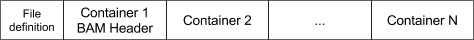
\includegraphics[width=356pt, height=31pt, keepaspectratio=true]{img/CRAMFileFormat2-1-fig001.png}
%%\caption{This should be the caption for \texttt{img/CRAMFileFormat2-1-fig001.png}.}
%%\end{figure}

Pic.1 CRAM file starts with a file definition followed by the BAM header and other 
containers.

Containers consist of one or more blocks. By convention, the BAM header is stored 
in the first container within a single block. This is known as the BAM header block.

%%\begin{figure}[htbp]
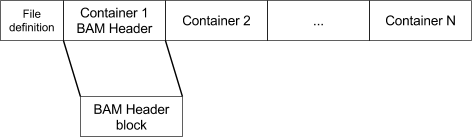
\includegraphics[width=354pt, height=103pt, keepaspectratio=true]{img/CRAMFileFormat2-1-fig002.png}
%%\caption{This should be the caption for \texttt{img/CRAMFileFormat2-1-fig002.png}.}
%%\end{figure}

Pic.2 The BAM header is stored in the first container.

Each container starts with a container header followed by one or more blocks. Each 
block starts with a block header. All data in CRAM is stored within blocks after 
the block header.

%%\begin{figure}[htbp]
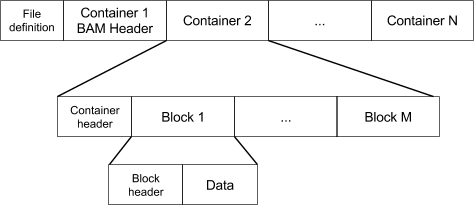
\includegraphics[width=356pt, height=154pt, keepaspectratio=true]{img/CRAMFileFormat2-1-fig003.png}
%%\caption{This should be the caption for \texttt{img/CRAMFileFormat2-1-fig003.png}.}
%%\end{figure}

Pic.3 Container and block structure. All data in CRAM files is stored in blocks.

The first block in each container is the compression header block:

%%\begin{figure}[htbp]
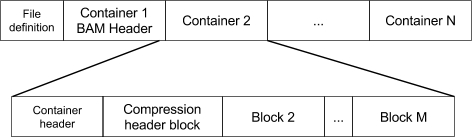
\includegraphics[width=354pt, height=103pt, keepaspectratio=true]{img/CRAMFileFormat2-1-fig004.png}
%%\caption{This should be the caption for \texttt{img/CRAMFileFormat2-1-fig004.png}.}
%%\end{figure}

Pic.4 Compression header is the first block in the container.

The blocks after the compression header are organised logically into slices. One 
slice may contain, for example, a contiguous region of alignment data. Slices begin 
with a slice header block and are followed by one or more data blocks:

%%\begin{figure}[htbp]
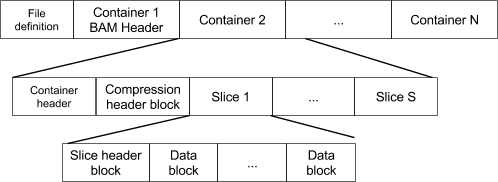
\includegraphics[width=374pt, height=137pt, keepaspectratio=true]{img/CRAMFileFormat2-1-fig005.png}
%%\caption{This should be the caption for \texttt{img/CRAMFileFormat2-1-fig005.png}.}
%%\end{figure}

Pic.5 Containers are logically organised into slices.

Data blocks are divided into core and external data blocks. Each slice must have 
at least one core data block immediately after the slice header block. The core 
data block may be followed by one or more external data blocks.

%%\begin{figure}[htbp]
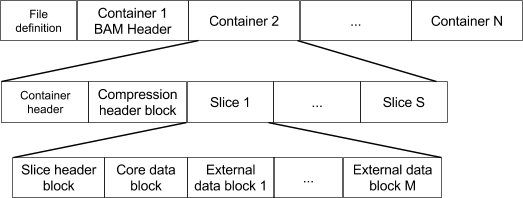
\includegraphics[width=392pt, height=149pt, keepaspectratio=true]{img/CRAMFileFormat2-1-fig006.png}
%%\caption{This should be the caption for \texttt{img/CRAMFileFormat2-1-fig006.png}.}
%%\end{figure}

Pic.5 Data blocks are divided into core and external data blocks. 

\section{\textbf{File definition}}

Each CRAM file starts with a fixed length (26 bytes) definition with the following 
fields:

\begin{tabular}{|l|l|l|}
\hline
\textbf{Data type} & \textbf{Name} & \textbf{Value}\tabularnewline
\hline
byte[4] & format magic number & CRAM (0x43 0x52 0x41 0x4d)\tabularnewline
\hline
unsigned byte & major format number & 2 (0x2)\tabularnewline
\hline
unsigned byte & minor format number & 0 (0x0)\tabularnewline
\hline
byte[20] & file id & CRAM file identifier (e.g. file name or SHA1 checksum)\tabularnewline
\hline
\end{tabular}

\section{\textbf{Container structure}}

The file definition is followed by one or more containers with the following header 
structure where the container content is stored in the `blocks' field:

\begin{tabular}{|l|>{\raggedright}p{120pt}|>{\raggedright}p{260pt}|}
\hline
\textbf{Data type} & \textbf{Name} & \textbf{Value}
\tabularnewline
\hline
int32 & length & byte size of the container data (blocks)\tabularnewline
\hline
itf8 & reference sequence id & reference sequence identifier  or\linebreak{}
-1 for unmapped reads\linebreak{}
-2 for multiple reference sequences\tabularnewline
\hline
itf8 & starting position on the reference & the alignment start position or\linebreak{}
0 for unmapped reads\tabularnewline
\hline
itf8 & alignment span & the length of the alignment or\linebreak{}
0 for unmapped reads\tabularnewline
\hline
itf8 & number of records & number of records in the container\tabularnewline
\hline
itf8 & record counter & 1-based sequential index of records in the file/stream.\tabularnewline
\hline
ltf8 & bases & number of read bases\tabularnewline
\hline
itf8 & number of blocks & the number of blocks\tabularnewline
\hline
itf8[ ] & landmarks & Each integer value of this array is a byte offset into the 
blocks byte array. Landmarks are used for random access indexing.\tabularnewline
\hline
byte[ ] & blocks & The blocks contained within the container.\tabularnewline
\hline
\end{tabular}

\subsection{\textbf{CRAM header in the first container}}

The first container in the CRAM file contains the BAM header in an uncompressed 
block.  BAM header is terminated with \textbackslash{}0 byte and any extra bytes 
in the block can be used to expand the BAM header. For example when updating @SQ 
records additional space may be required for the BAM header. It is recommended 
to reserve 50\% more space in the CRAM header block than it is required by the 
BAM header.

\section{\textbf{Block structure}}

Containers consist of one or more blocks. Block compression is applied independently 
and in addition to any encodings used to compress data within the block. The block 
have the following header structure with the data stored in the `block data' field:

\begin{tabular}{|l|>{\raggedright}p{120pt}|>{\raggedright}p{260pt}|}
\hline
\textbf{Data type} & \textbf{Name} & \textbf{Value}
\tabularnewline
\hline
byte & method & the block compression method: \linebreak{}
0: raw (none)*\linebreak{}
1: gzip\linebreak{}
2: bzip2\tabularnewline
\hline
byte & block content type id & the block content type identifier\tabularnewline
\hline
itf8 & block content id & the block content identifier used to associate external 
data blocks with data series\tabularnewline
\hline
itf8 & size in bytes* & size of the block data after applying block compression\tabularnewline
\hline
itf8 & raw size in bytes* & size of the block data before applying block compression\tabularnewline
\hline
byte[ ] & block data & the data stored in the block:\linebreak{}
$\bullet$ bit stream of CRAM records (core data block)\linebreak{}
$\bullet$ byte stream (external data block)\linebreak{}
$\bullet$ additional fields ( header blocks)\tabularnewline
\hline
\end{tabular}

* Note on raw method: both compressed and raw sizes must be set to the same value.

\subsection{\textbf{Block content types}}

CRAM has the following block content types:

\begin{tabular}{|>{\raggedright}p{143pt}|>{\raggedright}p{45pt}|>{\raggedright}p{116pt}|>{\raggedright}p{114pt}|}
\hline
\textbf{Block content type} & \textbf{Block content type id} & \textbf{Name} & \textbf{Contents}\tabularnewline
\hline
FILE\_HEADER & 0 & BAM header block & BAM header\tabularnewline
\hline
COMPRESSION\_HEADER & 1 & Compression header block & See specific section\tabularnewline
\hline
MAPPED\_SLICE\_HEADER & 2 & Slice header block & See specific section\tabularnewline
\hline
 & 3 &  & reserved\tabularnewline
\hline
EXTERNAL\_DATA & 4 & external data block & data produced by external encodings\tabularnewline
\hline
CORE\_DATA & 5 & core data block & bit stream of all encodings except for external\tabularnewline
\hline
\end{tabular}


\subsection{\textbf{Block content id}}

Block content id is used to distinguish between external blocks in the same slice. 
Each external encoding has an id parameter which must be one of the external block 
content ids. For external blocks the content id is a positive integer. For all 
other blocks content id should be 0. Consequently, all external encodings must 
not use content id less than 1. 

\subsubsection*{Data blocks}

Data is stored in data blocks. There are two types of data blocks: core data blocks 
and external data blocks.The difference between core and external data blocks is 
that core data blocks consist of data series that are compressed using bit encodings 
while the external data blocks are byte compressed. One core data block and any 
number of external data blocks are associated with each slice.

Writing to and reading from core and external data blocks is organised through 
CRAM records. Each data series is associated with an encoding. In case of external 
encoding the block content id is used to identify the block where the data series 
is stored. Please note that external blocks can have multiple data series associated 
with them; in this case the values from these data series will be interleaved. 


\subsection{\textbf{BAM header block}}

The BAM header is stored in a single block within the first container. 

The following constraints apply to the BAM header: 

\begin{itemize}
\item The SQ:MD5 checksum is required unless the reference sequence has been embedded 
into the file.

\item At least one RG record is required.

\item The HD:SO sort order is always POS.
\end{itemize}

\subsection{\textbf{Compression header block}}

The compression header block consists of 3 parts: preservation map, data series 
encoding map and tag encoding map.

\subsubsection*{Preservation map}

The preservation map contains information about which data was preserved in the 
CRAM file. It is stored as a map with byte[2] keys:

\begin{tabular}{|l|l|>{\raggedright}p{100pt}|>{\raggedright}p{220pt}|}
\hline
\textbf{Key} & \textbf{Value data type} & \textbf{Name} & \textbf{Value}\tabularnewline
\hline
RN & bool & read names included & true if read names are preserved for all reads\tabularnewline
\hline
AP & bool & AP data series delta & true if AP data series is delta, false otherwise\tabularnewline
\hline
RR & bool & reference required & true if reference sequence is required to restore 
the data completely\tabularnewline
\hline
SM & byte[5] & substitution matrix & substitution matrix\tabularnewline
\hline
TD & byte[ ] & tag ids dictionary & a list of lists of tag ids, see tag encoding 
section\tabularnewline
\hline
\end{tabular}

\subsubsection*{Data series encodings}

Each data series has an encoding. These encoding are stored in a map with byte[2] 
keys:

\begin{tabular}{|l|l|>{\raggedright}p{100pt}|>{\raggedright}p{220pt}|}
\hline
\textbf{Key} & \textbf{Value data type} & \textbf{Name} & \textbf{Value}\tabularnewline
\hline
BF & encoding\texttt{<}int\texttt{>} & bit flags & see separate section\tabularnewline
\hline
AP & encoding\texttt{<}int\texttt{>} & in-seq positions & 0-based alignment start 
delta from previous record *\tabularnewline
\hline
FP & encoding\texttt{<}int\texttt{>} & in-read positions & positions of the read 
features\tabularnewline
\hline
RL & encoding\texttt{<}int\texttt{>} & read lengths & read lengths\tabularnewline
\hline
DL & encoding\texttt{<}int\texttt{>} & deletion lengths & base-pair deletion lengths\tabularnewline
\hline
NF & encoding\texttt{<}int\texttt{>} & distance to next fragment & number of records 
to the next fragment*\tabularnewline
\hline
BA & encoding\texttt{<}byte\texttt{>} & bases & bases\tabularnewline
\hline
QS & encoding\texttt{<}byte\texttt{>} & quality scores & quality scores\tabularnewline
\hline
FC & encoding\texttt{<}byte\texttt{>} & read features codes & see separate section\tabularnewline
\hline
FN & encoding\texttt{<}int\texttt{>} & number of read features & number of read 
features in each record\tabularnewline
\hline
BS & encoding\texttt{<}byte\texttt{>} & base substitution codes & base substitution 
codes\tabularnewline
\hline
IN & encoding\texttt{<}byte[ ]\texttt{>} & insertion & inserted bases\tabularnewline
\hline
RG & encoding\texttt{<}int\texttt{>} & read groups & read groups. Special value 
`-1' stands for no group.\tabularnewline
\hline
MQ & encoding\texttt{<}int\texttt{>} & mapping qualities & mapping quality scores 
 \tabularnewline
\hline
TL & encoding\texttt{<}int\texttt{>} & tag ids  & list of tag ids, see tag encoding 
section\tabularnewline
\hline
RN & encoding\texttt{<}byte[ ]\texttt{>} & read names & read names\tabularnewline
\hline
NS & encoding\texttt{<}int\texttt{>} & next fragment reference sequence id & reference 
sequence ids for the next fragment \tabularnewline
\hline
NP & encoding\texttt{<}int\texttt{>} & next mate alignment start & alignment positions 
for the next fragment\tabularnewline
\hline
TS & encoding\texttt{<}int\texttt{>} & template size & template sizes\tabularnewline
\hline
MF & encoding\texttt{<}int\texttt{>} & next mate bit flags & see specific section\tabularnewline
\hline
CF & encoding\texttt{<}int\texttt{>} & compression bit flags & see specific section\tabularnewline
\hline
TM & encoding\texttt{<}int\texttt{>} & test mark & a prefix expected before every 
record, for debugging purposes.\tabularnewline
\hline
RI & encoding\texttt{<}int\texttt{>} & reference id & record reference id from 
the BAM file header\tabularnewline
\hline
RS & encoding\texttt{<}int\texttt{>} & reference skip length & number of skipped 
bases for the `N' read feature\tabularnewline
\hline
PD & encoding\texttt{<}int\texttt{>} & padding & number of padded bases\tabularnewline
\hline
HC & encoding\texttt{<}int\texttt{>} & hard clip & number of hard clipped bases\tabularnewline
\hline
SC & encoding\texttt{<}byte[ ]\texttt{>} & soft clip & soft clipped bases\tabularnewline
\hline
\end{tabular}

* The data series is reset for each slice. 

\subsubsection*{Encoding tags}

The TL (tag list) data series represents combined information about the number 
of tags in a record and their ids. 

Let $L_{i}=\{T_{i0}, T_{i1}, \ldots, T_{ix}\}$
be sorted list of all tag ids for a record $R_{i}$, where $i$ is the sequential 
record index and $T_{ij}$ denotes $j$-th tag id in the record. We recommend 
alphabetical sort order. The list of unique $L_{i}$ is assigned sequential 
integer numbers starting with 0. These integer numbers represent the TL data series. 
The sorted list of unique $L_{i}$ is stored as the TD value in the preservation 
map. Using TD, an integer from the TL data series can be mapped back into a list 
of tag ids. 

The TD is written as byte array consisting of $L_{i}$ values separated 
with \textbackslash{}0. Each $L_{i}$ value is written as a sequence 
of 3 bytes: tag id followed by tag value type. For example AMiOQz\textbackslash{}0OQz\textbackslash{}0, 
where the TD consists of just two values: integer 0 for tags \{AM:i,OQ:z\} and 
1 for tag \{OQ:z\}.

\subsubsection*{Encoding tag values}

The encodings used for different tags are stored in a map. The map has integer 
keys composed of the two letter tag abbreviation followed by the tag type as defined 
in the SAM specification, for example `OQZ' for `OQ:Z'. The three bytes form a 
big endian integer and are written as ITF8. For example, 3-byte representation 
of OQ:Z is \{0x4F, 0x51, 0x5A\} and these bytes are intepreted as the integer 0x004F515A. 
The integer is finally written as ITF8.

\begin{tabular}{|l|l|l|>{\raggedright}p{160pt}|}
\hline
\textbf{Key} & \textbf{Value data type} & \textbf{Name} & \textbf{Value}
\tabularnewline
\hline
TAG NAME 1:TAG TYPE 1 & encoding\texttt{<}byte[ ]\texttt{>} & read tag 1 & tag values 
(names and types are available in the data series code)\tabularnewline
\hline
... &  & ... & ...\tabularnewline
\hline
TAG NAME N:TAG TYPE N & encoding\texttt{<}byte[ ]\texttt{>} & read tag N & ...\tabularnewline
\hline
\end{tabular}

Note that tag values are encoded as array of bytes. The routines to convert tag 
values into byte array and back are the same as in BAM with the exception of value 
type being captured in the tag key rather in the value. 

\subsection{\textbf{Slice header block}}

The slice header block is never compressed (block method=raw). For reference mapped 
reads the slice header also defines the reference sequence context of the data 
blocks associated with the slice. Mapped and unmapped reads can be stored within 
the same slice similarly to BAM file. Slices with unsorted reads must not contain 
any other types of reads.

The slice header block contains the following fields.

\begin{tabular}{|l|l|>{\raggedright}p{200pt}|}
\hline
\textbf{Data type} & \textbf{Name} & \textbf{Value}\tabularnewline
\hline
itf8 & reference sequence id & reference sequence identifier or -1 for unmapped 
or unsorted reads\tabularnewline
\hline
itf8 & alignment start & the alignment start position or -1 for unmapped or unsorted 
reads\tabularnewline
\hline
itf8 & alignment span & the length of the alignment or 0 for unmapped or unsorted 
reads\tabularnewline
\hline
itf8 & number of records & the number of records in the slice\tabularnewline
\hline
ltf8 & record counter & 1-based sequential index of records in the file/stream\tabularnewline
\hline
itf8 & number of blocks & the number of blocks in the slice\tabularnewline
\hline
itf8[ ] & block content ids & block content ids of the blocks in the slice\tabularnewline
\hline
itf8 & embedded reference bases block content id & block content id for the embedded 
reference sequence bases or -1 for none\tabularnewline
\hline
byte[16] & reference md5 & MD5 checksum of the reference bases within the slice 
boundaries or 16 \textbackslash{}0 bytes for unmapped or unsorted reads\tabularnewline
\hline
\end{tabular}

\subsection{\textbf{Core data block}}

A core data block is a bit stream (most significant bit first) consisting of one 
or more CRAM records. Please note that one byte could hold more then one CRAM record 
as a minimal CRAM record could be just a few bits long. The core data block has 
the following fields:

\begin{tabular}{|l|>{\raggedright}p{120pt}|>{\raggedright}p{260pt}|}
\hline
\textbf{Data type} & \textbf{Name} & \textbf{Value}
\tabularnewline
\hline
bit[ ] & CRAM record 1 & The first CRAM record\tabularnewline
\hline
... & ... & ...\tabularnewline
\hline
bit[ ] & CRAM record N & The Nth CRAM record \tabularnewline
\hline
\end{tabular}

\subsection{\textbf{External data block}}

Relationship between core data block and external data blocks is shown in the following 
picture: 

%%\begin{figure}[htbp]
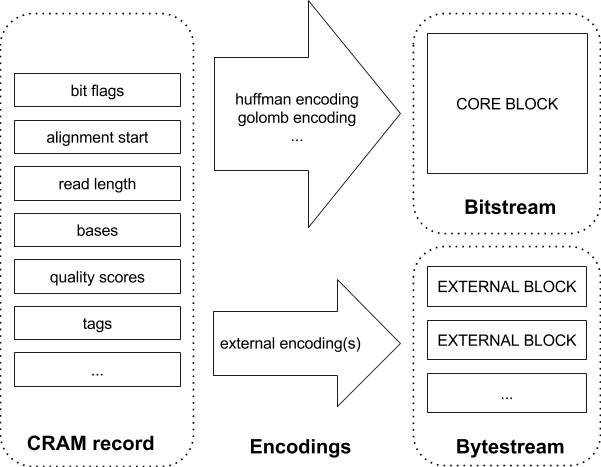
\includegraphics[width=451pt, height=350pt, keepaspectratio=true]{img/CRAMFileFormat2-1-fig007.png}
%%\caption{This should be the caption for \texttt{img/CRAMFileFormat2-1-fig007.png}.}
%%\end{figure}

Pic.3 Relationship between core data block and external data blocks.

The picture shows how a CRAM record (on the left) is partially written to core 
data block while the other fields are stored in two external data blocks. The specific 
encodings are presented only for demonstration purposes, the main point here is 
to distinguish between bit encodings whose output is always stored in core data 
block and the external encoding which simply stored the bytes into external data 
blocks.

\section{\textbf{End of file marker}}

A special container is used to mark the end of a file or stream. It is optional 
in version preceding 2.1 but required in later versions. The idea is to provide 
an easy and a quick way to detect that a CRAM file or stream is complete. The marker 
is basically an empty container with ref seq id set to -1 (unaligned) and alignment 
start set to 4542278.

Here is a complete content of the EOF container explained in detail:

\begin{tabular}{|l|l|>{\raggedright}p{150pt}|>{\raggedright}p{180pt}|}
\hline
\textbf{hex bytes} & \textbf{data type} & \textbf{decimal value} & \textbf{field 
name}\tabularnewline
\hline
\multicolumn{4}{|l|}{\textit{Container header}}\tabularnewline
\hline
0b 00 00 00 & integer & 11 & size of blocks data\tabularnewline
\hline
ff ff ff ff ff & itf8 & -1 & ref seq id\tabularnewline
\hline
e0 45 4f 46 & itf8 & 4542278 & alignment start\tabularnewline
\hline
00 & itf8 & 0 & alignment span\tabularnewline
\hline
00 & itf8 & 0 & nof records\tabularnewline
\hline
00 & itf8 & 0 & global record counter\tabularnewline
\hline
00 & itf8 & 0 & bases\tabularnewline
\hline
01 & itf8 & 1 & block count\tabularnewline
\hline
00 & array & 0 & landmarks\tabularnewline
\hline
\multicolumn{4}{|l|}{\textit{Compression header block}}\tabularnewline
\hline
00 & byte & 0 (RAW) & compression method\tabularnewline
\hline
01 & byte & 1 (COMPRESSION\_HEADER) & block content type\tabularnewline
\hline
00 & itf8 & 0 & block content id\tabularnewline
\hline
06 & itf8 & 6 & compressed size\tabularnewline
\hline
06 & itf8 & 6 & uncompressed size\tabularnewline
\hline
\multicolumn{4}{|l|}{\textit{Compression header}}\tabularnewline
\hline
01 & itf8 & 1 & preservation map byte size\tabularnewline
\hline
00 & itf8 & 0 & preservation map size\tabularnewline
\hline
01 & itf8 & 1 & encoding map byte size\tabularnewline
\hline
00 & itf8 & 0 & encoding map size\tabularnewline
\hline
01 & itf8 & 1 & tag encoding byte size\tabularnewline
\hline
00 & itf8 & 0 & tag encoding map size\tabularnewline
\hline
\end{tabular}

When compiled together the EOF marker is exactly 30 bytes long and in hex representation 
is:

0b 00 00 00 ff ff ff ff ff e0 45 4f 46 00 00 00 00 01 00  00 01 00 06 06 01 00 
01 00 01 00

\section{\textbf{Record structure}}

CRAM record is based on the SAM record but has additional features allowing for 
more efficient data storage.  In contrast to BAM record CRAM record uses bits as 
well as bytes for data storage. This way, for example, various coding techniques 
which output variable length binary codes can be used directly in CRAM. On the 
other hand, data series that do not require binary coding can be stored separately 
in external blocks with some other compression applied to them independently.

\subsection{\textbf{CRAM record}}

Both mapped and unmapped reads start with the following fields. Please note that 
the data series type refers to the logical data type and the data series name corresponds 
to the data series encoding map.

\begin{tabular}{|>{\raggedright}p{36pt}|>{\raggedright}p{70pt}|>{\raggedright}p{75pt}|>{\raggedright}p{90pt}|>{\raggedright}p{171pt}|}
\hline
 & \textbf{Data series type} & \textbf{Data series name} & \textbf{Field} & \textbf{Description}\tabularnewline
\hline
1 & int & BF & CRAM bit flags & see CRAM record bit flags\tabularnewline
\hline
2 & int & CF  & compression bit flags & see compression bit flags\tabularnewline
\hline
3 & int & RI & ref id & reference sequence id, not used for single reference slices, 
reserved for future multiref slices. \tabularnewline
\hline
4 & int & RL & read length & the length of the read\tabularnewline
\hline
5 & int & AP & alignment start & the alignment start position *1\tabularnewline
\hline
6 & int & RG & read group & the read group identifier\tabularnewline
\hline
7 & byte & QS & quality scores & quality scores are stored depending on the value 
of the `mapped QS included' field\tabularnewline
\hline
8 & byte[ ] & RN & read name & the read names (if preserved)\tabularnewline
\hline
9 & *2 & *2 & mate record & *2 (if not the last record)\tabularnewline
\hline
10 & int & TL & tag ids & tag ids *3\tabularnewline
\hline
11 & byte[ ] & - & tag values & tag values *3\tabularnewline
\hline
\end{tabular}

*1 The AP data series is delta encoded for reads mapped to a single reference slice 
and normal integer value in all other cases. 

*2 See \emph{mate record} section.

*3 See\emph{ tag encoding} section.

The CRAM record structure for mapped reads has the following additional fields:

\begin{tabular}{|>{\raggedright}p{36pt}|>{\raggedright}p{70pt}|>{\raggedright}p{74pt}|>{\raggedright}p{85pt}|>{\raggedright}p{177pt}|}
\hline
 & \textbf{Data series type} & \textbf{Data series name} & \textbf{Field} & \textbf{Description}\tabularnewline
\hline
1 & *1 & *1 & read feature records & *1\tabularnewline
\hline
2 & byte & MQ & mapping quality & read mapping quality\tabularnewline
\hline
\end{tabular}

*1 See read feature record specification below.

The CRAM record structure for unmapped reads has the following additional fields:

\begin{tabular}{|>{\raggedright}p{8pt}|>{\raggedright}p{88pt}|>{\raggedright}p{83pt}|>{\raggedright}p{85pt}|>{\raggedright}p{178pt}|}
\hline
 & \textbf{Data series type} & \textbf{Data series name} & \textbf{Field} & \textbf{Description}\tabularnewline
\hline
1 & byte[read length] & BA & bases & the read bases\tabularnewline
\hline
\end{tabular}

\subsection{\textbf{Read bases}}

CRAM format supports ACGTN bases only. All non-ACGTN read bases must be replaced 
with N (unknown) base. In case of mismatching non-ACGTN read base and non-ACGTN 
reference base a ReadBase read feature should be used to capture the fact that 
the read base should be restored as N base. 

\subsection{\textbf{CRAM record bit flags (BF data series)}}

The following flags are defined for each CRAM read record:

\begin{tabular}{|>{\raggedright}p{144pt}|>{\raggedright}p{144pt}|>{\raggedright}p{144pt}|}
\hline
\textbf{Bit flag} & \textbf{Comment} & \textbf{Description}\tabularnewline
\hline
0x1 & ! 0x40 \&\& ! 0x80 & template having multiple segments in sequencing\tabularnewline
\hline
0x2 &  & each segment properly aligned according to the aligner\tabularnewline
\hline
0x4 &  & segment unmapped\tabularnewline
\hline
0x8 & calculated* or stored in the mate's info & next segment in the template unmapped\tabularnewline
\hline
0x10 &  & SEQ being reverse complemented\tabularnewline
\hline
0x20 & calculated* or stored in the mate's info & SEQ of the next segment in the 
template being reversed\tabularnewline
\hline
0x40 &  & the first segment in the template\tabularnewline
\hline
0x80 &  & the last segment in the template\tabularnewline
\hline
0x100 &  & secondary alignment\tabularnewline
\hline
0x200 &  & not passing quality controls\tabularnewline
\hline
0x400 &  & PCR or optical duplicate\tabularnewline
\hline
\end{tabular}

* For segments within the same slice.

\subsection{\textbf{Read feature records}}

Read features are used to store read details that are expressed using read coordinates 
(e.g. base differences respective to the reference sequence). The read feature 
records start with the number of read features followed by the read features themselves:

\begin{tabular}{|>{\raggedright}p{36pt}|>{\raggedright}p{65pt}|>{\raggedright}p{84pt}|>{\raggedright}p{90pt}|>{\raggedright}p{168pt}|}
\hline
 & \textbf{Data series type} & \textbf{Data series name} & \textbf{Field} & \textbf{Description}\tabularnewline
\hline
1 & int & FN & number of read features & the number of read features\tabularnewline
\hline
2 *1 & int & FP & in-read-position & position of the read feature\tabularnewline
\hline
3 *1 & byte & FC & read feature code & *2\tabularnewline
\hline
4 *1 & *2 & *2 & read feature data & *2\tabularnewline
\hline
\end{tabular}

*1 Repeated for each read feature.

*2 See \emph{read feature codes} below.

\subsubsection*{Read feature codes}

The following codes are used to distinguish variations in read coordinates:

\begin{tabular}{|>{\raggedright}p{91pt}|>{\raggedright}p{45pt}|>{\raggedright}p{72pt}|>{\raggedright}p{66pt}|>{\raggedright}p{132pt}|}
\hline
\textbf{Feature code} & \textbf{Id} & \textbf{Data series type} & \textbf{Data 
series name} & \textbf{Description}\tabularnewline
\hline
Read base & B (0x42) & byte,byte & BA,QS & A base and associated quality score\tabularnewline
\hline
Substitution & X (0x58) & byte & BS & base substitution codes, SAM operators X, 
M and =\tabularnewline
\hline
Insertion & I (0x49) & byte[ ] & IN & inserted bases, SAM operator I\tabularnewline
\hline
Deletion & D (0x44) & int & DL & number of deleted bases, SAM operator D\tabularnewline
\hline
Insert base & i (0x69) & byte & BA & single inserted base, SAM operator I\tabularnewline
\hline
Quality score & Q (0x51) & byte & QS & single quality score\tabularnewline
\hline
Reference skip & N (0x4E) & int & RS & number of skipped bases, SAM operator N\tabularnewline
\hline
Soft clip & S & byte[ ] & SC & soft clipped bases, SAM operator S\tabularnewline
\hline
Padding & P & int & PD & number of padded bases, SAM operator P\tabularnewline
\hline
Hard clip & H & int & HC & number of hard clipped bases, SAM operator H\tabularnewline
\hline
\end{tabular}

\subsubsection*{Base substitution codes (BS data series)}

A base substitution is defined as a change from one nucleotide base (reference 
base) to another (read base) including N as an unknown or missing base. There are 
5 possible bases ACGTN, 4 possible substitutions for each base and 20 substitutions 
in total. Substitutions for the same reference base are assigned integer codes 
from 0 to 3 inclusive. To restore a base one would need to know its substitution 
code and the reference base. 

A base substitution matrix assigns integer codes to all possible substitutions. 

Substitution matrix is written as follows. Substitutions for a given reference 
base are sorted by their frequencies in descending order then assigned numbers 
from 0 to 3. Same-frequency ties are broken using alphabetical order. For example, 
let us assume the following substitution frequencies for base A: 

AC: 15\%

AG: 25\%

AT: 55\%

AN: 5\%

Then the substitution codes are: 

AC: 2

AG: 1

AT: 0

AN: 3

and they are written as a single byte, 10 01 00 11 = 147 decimal or 0x93 in this 
case. The whole substitution matrix is written as 5 bytes, one for each reference 
base in the alphabetical order: A, C, G, T and N.

Note: the last two bits of each substitution code are redundant but still required 
to simplify the reading. 

\subsection{\textbf{Mate record}}

There are two ways in which mate information can be preserved in CRAM: number of 
records downstream (distance) to the next fragment in the template and a special 
mate record if the next fragment is not in the current slice. Combination of the 
two approaches allows to fully restore BAM level mate information and efficiently 
store it in the CRAM file. 

For mates within the slice only the distance is captured:

\begin{tabular}{|>{\raggedright}p{7pt}|>{\raggedright}p{68pt}|>{\raggedright}p{115pt}|>{\raggedright}p{228pt}|}
\hline
 & \textbf{Data series type} & \textbf{Data series name} & \textbf{Description}\tabularnewline
\hline
1 & int & NF & the number of records to the next fragment\tabularnewline
\hline
\end{tabular}

If the next fragment is not found within the horizon then the following structure 
is included into the CRAM record:

\begin{tabular}{|>{\raggedright}p{6pt}|>{\raggedright}p{66pt}|>{\raggedright}p{117pt}|>{\raggedright}p{228pt}|}
\hline
 & \textbf{Data series type} & \textbf{Data series name} & \textbf{Description}\tabularnewline
\hline
1 & byte & MF & next mate bit flags, see table below\tabularnewline
\hline
2 & byte[ ] & RN & the read name\tabularnewline
\hline
3 & int & NS & mate reference sequence identifier \tabularnewline
\hline
4 & long & NP & mate alignment start position \tabularnewline
\hline
5 & int & TS & the size of the template (insert size)\tabularnewline
\hline
\end{tabular}

\subsubsection*{}

\subsubsection*{Next mate bit flags (MF data series)}

The next mate bit flags expressed as an integer represent the MF data series. The 
following bit flags are defined:

\begin{tabular}{|>{\raggedright}p{47pt}|>{\raggedright}p{134pt}|>{\raggedright}p{250pt}|}
\hline
\textbf{Bit flag} & \textbf{Name} & \textbf{Description}\tabularnewline
\hline
0x1 & mate negative strand bit & the bit is set if the mate is on the negative 
strand\tabularnewline
\hline
0x2 & mate mapped bit & the bit is set if the mate is mapped\tabularnewline
\hline
\end{tabular}

\subsubsection*{Read names (RN data series)}

Read names can be preserved in the CRAM format. However, it is anticipated that 
in the majority of cases original read names will not be preserved and sequential 
integer numbers will be used as read names. Read names may also be used to associate 
fragments into templates when the fragments are too far apart to be referenced 
by the number of CRAM records. In this case the read names are not required to 
be the same as the original ones. Their only two requirements are:

$\bullet$ read name must be the same for all fragments of the same template

$\bullet$ read name of a template must be unique within a file

\subsection{\textbf{Compression bit flags (CF data series)}}

The compression bit flags expressed as an integer represent the CF data series. 
The following compression flags are defined for each CRAM read record:

\begin{tabular}{|>{\raggedright}p{39pt}|>{\raggedright}p{150pt}|>{\raggedright}p{242pt}|}
\hline
\textbf{Bit flag} & \textbf{Name} & \textbf{Description}\tabularnewline
\hline
0x1 & quality scores stored as array & quality scores can be stored as read features 
or as an array similar to read bases.\tabularnewline
\hline
0x2 & detached & the next segment is out of horizon\tabularnewline
\hline
0x4 & has mate downstream & tells if the next segment should be expected further 
in the stream\tabularnewline
\hline
\end{tabular}

\section{\textbf{Reference sequences}}

CRAM format is natively based upon usage of reference sequences even though in 
some cases they are not required. In contrast to BAM format CRAM format has strict 
rules about reference sequences. 

\begin{enumerate}
\item M5 (sequence MD5 checksum) field of @SQ sequence record in the BAM header is 
required and UR (URI for the sequence fasta optionally gzipped file) field is strongly 
advised. The rule for calculating MD5 is to remove any non-base symbols (like \textbackslash{}n, 
sequence name or length and spaces) and upper case the rest. Here are some examples: 

\texttt{> samtools faidx human\_g1k\_v37.fasta 1 \textbar{} grep -v '\textasciicircum{}>' \textbar{} tr -d '\textbackslash{}n' \textbar{} tr a-z A-Z \textbar{} md5sum -\\
1b22b98cdeb4a9304cb5d48026a85128  -}

\texttt{> samtools faidx human\_g1k\_v37.fasta 1:10-20 \textbar{}grep -v '\textasciicircum{}\texttt{>}' \textbar{}tr -d '\textbackslash{}n' \textbar{}tr a-z A-Z \textbar{}md5sum -\\
0f2a4865e3952676ffad2c3671f14057  -}

Please note that the latter calculates the checksum for 11 bases from position 
10 (inclusive) to 20 (inclusive) and the bases are counted 1-based, so the first 
base position is 1. 

\item All CRAM reader implementations are expected to check for reference MD5 checksums 
and report any missing or mismatching entries. Consequently, all writer implementations 
are expected to ensure that all checksums are injected or checked during compression 
time. 

\item In some cases reads may be mapped beyond the reference sequence. All out of 
range reference bases are all assumed to be `N'. 

\item MD5 checksum bytes in slice header should be ignored for unmapped or multiref 
slices. 
\end{enumerate}

\section{\textbf{Indexing}}

\subsubsection*{General notes}

Please note that CRAM indexing is external to the file format itself and may change 
independently of the file format specification in the future. For example, a new 
type of index files may appear. 

Individual records are not indexed in CRAM files, slices should be used instead 
as a unit of random access. Another important difference between CRAM and BAM indexing 
is that CRAM container header and compression header block (first block in container) 
must always be read before decoding a slice. Therefore two read operations are 
required for random access in CRAM.

Indexing a CRAM file is deemed to be a lightweight operation because it does not 
require any CRAM records to be read. All indexing information can be obtained from 
container headers, namely sequence id, alignment start and span, container start 
byte offset and slice byte offset inside the container. 

\subsubsection*{CRAM index}

A CRAM index is a gzipped tab delimited file containing the following columns:

\begin{enumerate}
\item Sequence id

\item Alignment start

\item Alignment span

\item Container start byte offset in the file

\item Slice start byte offset in the container data (`blocks')

\item Slice bytes
\end{enumerate}

Each line represents a slice in the CRAM file. Please note that all slices must 
be listed in index file.

\subsubsection*{BAM index}

BAM indexes are supported by using 4-byte integer pointers called landmarks that 
are stored in container header. BAM index pointer is a 64-bit value with 48 bits 
reserved for the BAM block start position and 16 bits reserved for the in-block 
offset. When used to index CRAM files, the first 48 bits are used to store the 
CRAM container start position and the last 16 bits are used to store the index 
of the landmark in the landmark array stored in  container header. The landmark 
index can be used to access the appropriate slice. 

The above indexing scheme treats CRAM slices as individual records in BAM file. 
This allows to apply BAM indexing to CRAM files, however it introduces some overhead 
in seeking specific alignment start because all preceding records in the slice 
must be read and discarded.

\section{\textbf{Appendix}}

\subsection{\textbf{External encoding}}

External encoding operates on bytes only. Therefore any data series must be translated 
into bytes before sending data into an external block. The following agreements 
are defined. 

Integer values are written as ITF8, which then can be translated into an array 
of bytes. 

Strings, like read name, are translated into bytes according to UTF8 rules. In 
most cases these should coincide with ASCII, making the translation trivial. 

\subsection{\textbf{Codings}}

\subsubsection*{Introduction}

The basic idea for codings is to efficiently represent some values in binary format. 
This can be achieved in a number of ways that most frequently involve some knowledge 
about the nature of the values being encoded, for example, distribution statistics. 
The methods for choosing the best encoding and determining its parameters are very 
diverse and are not part of the CRAM format specification, which only describes 
how the information needed to decode the values should be stored.

\subsubsection*{Offset}

Most of the codings listed below encode positive integer numbers. An integer offset 
value is used to allow any integer numbers and not just positive ones to be encoded. 
It can also be used for monotonically decreasing distributions with the maximum 
not equal to zero. For example, given offset is 10 and the value to be encoded 
is 1, the actually encoded value would be offset+value=11. Then when decoding, 
the offset would be subtracted from the decoded value. 

\subsubsection*{Beta coding}

\subsubsection*{Definition}

Beta coding is a most common way to represent numbers in \emph{binary notation}. 


\subsubsection*{Examples}

\begin{tabular}{|>{\raggedright}p{222pt}|>{\raggedright}p{222pt}|}
\hline
\textbf{Number} & \textbf{Codeword}\tabularnewline
\hline
0 & 0\tabularnewline
\hline
1 & 1\tabularnewline
\hline
2 & 10\tabularnewline
\hline
4 & 100\tabularnewline
\hline
\end{tabular}

\subsubsection*{Parameters}

CRAM format defines the following parameters of beta coding: 

\begin{tabular}{|>{\raggedright}p{144pt}|>{\raggedright}p{144pt}|>{\raggedright}p{144pt}|}
\hline
\textbf{Data type} & \textbf{Name} & \textbf{Comment}\tabularnewline
\hline
itf8 & offset & offset is added to each value\tabularnewline
\hline
itf8 & length & the number of bits used\tabularnewline
\hline
\end{tabular}

\subsubsection*{Gamma coding}

\subsubsection*{Definition}

\emph{Elias gamma code} is a prefix encoding of positive integers. This is a combination 
of unary coding and beta coding. The first is used to capture the number of bits 
required for beta coding to capture the value. 

\subsubsection*{Encoding}

\begin{enumerate}
\item Write it in binary.

\item Subtract $1$ from the number of bits written in step 1 and prepend that many zeros.

\item An equivalent way to express the same process:

\item Separate the integer into the highest power of $2$ it contains ($2N$) and the remaining 
$N$ binary digits of the integer.

\item Encode $N$ in unary; that is, as $N$ zeroes followed by a one.

\item Append the remaining $N$ binary digits to this representation of $N$.
\end{enumerate}

\subsubsection*{Decoding}

\begin{enumerate}
\item Read and count 0s from the stream until you reach the first 1. Call this count 
of zeroes $N$.

\item Considering the one that was reached to be the first digit of the integer, with 
a value of $2N$, read the remaining $N$ digits of the integer.
\end{enumerate}

\subsubsection*{Examples}

\begin{tabular}{|>{\raggedright}p{76pt}|>{\raggedright}p{107pt}|}
\hline
\textbf{Value} & \textbf{Codeword}\tabularnewline
\hline
1 & 1\tabularnewline
\hline
2 & 010\tabularnewline
\hline
3 & 011\tabularnewline
\hline
4 & 00100\tabularnewline
\hline
\end{tabular}

\subsubsection*{Parameters}

\begin{tabular}{|>{\raggedright}p{144pt}|>{\raggedright}p{144pt}|>{\raggedright}p{144pt}|}
\hline
\textbf{Data type} & \textbf{Name} & \textbf{Comment}\tabularnewline
\hline
itf8 & offset & offset is added to each value\tabularnewline
\hline
\end{tabular}

\subsubsection*{Golomb coding}

\subsubsection*{Definition}

\emph{Golomb encoding} is a prefix encoding optimal for representation of random 
positive numbers following geometric distribution. 

\begin{enumerate}
\item Fix the parameter $M$ to an integer value.

\item For $N$, the number to be encoded, find

\begin{enumerate}
\item quotient $q = \lfloor N/M \rfloor$

\item remainder $r = N \bmod M$
\end{enumerate}

\item Generate Codeword

\begin{enumerate}
\item The Code format : \texttt{<}Quotient Code\texttt{>}\texttt{<}Remainder Code\texttt{>}, 
where

\item Quotient Code (in unary coding)

\begin{enumerate}
\item Write a $q$-length string of 1 bits

\item Write a 0 bit
\end{enumerate}

\item Remainder Code (in truncated binary encoding)

\begin{enumerate}
\item If $M$ is power of 2, code remainder as binary format. So $log_{2}(M)$ bits are needed. (Rice code)  

\item If $M$ is not a power of 2, set $b=\lceil log_{2}(M) \rceil$

\begin{enumerate}
\item If $r < 2^{b}-M$ code $r$ as plain binary using $b-1$ bits.

\item If $r \ge 2^{b}$ code the number $r+2^{b}$ in plain binary representation 
using $b$ bits.
\end{enumerate}
\end{enumerate}
\end{enumerate}
\end{enumerate}

\subsubsection*{Examples}

\begin{tabular}{|>{\raggedright}p{76pt}|>{\raggedright}p{107pt}|}
\hline
\textbf{Number} & \textbf{Codeword, M=10}\tabularnewline
\hline
0 & 0000\tabularnewline
\hline
4 & 0100\tabularnewline
\hline
10 & 10000\tabularnewline
\hline
42 & 11110010\tabularnewline
\hline
\end{tabular}

\subsubsection*{Parameters}

Golomb coding takes the following parameters: 

\begin{tabular}{|>{\raggedright}p{144pt}|>{\raggedright}p{144pt}|>{\raggedright}p{144pt}|}
\hline
\textbf{Data type} & \textbf{Name} & \textbf{Comment}\tabularnewline
\hline
itf8 & offset & offset is added to each value\tabularnewline
\hline
itf8 & M & the golomb parameter (number of bins)\tabularnewline
\hline
\end{tabular}

\subsubsection*{Golomb-Rice coding}

Golomb-Rice coding is a special case of Golomb coding when the M parameter is a 
power of 2. The reason for this coding is that the division operations in Golomb 
coding can be replaced with bit shift operators. 

\subsubsection*{Subexponential coding}

\subsubsection*{Definition}

Subexponential coding is parametrized by a non-nengative integer $k$. The 
main feature of the subexponential code is its length. For integers $n < 2k+1$
the code length increases linearly with $n$, but for larger $n$ 
it increases logarithmically.

\subsubsection*{Encoding}

\begin{enumerate}
\item Determine the group index i using the following rules: 

\begin{enumerate}
\item if $n < 2^{k}$, then $i = 0$. 

\item if $n \ge 2^{k}$ , then determine $i$ such that $2^{i+k-1} \le n < 2^{i+k}$
\end{enumerate}

\item Form the prefix of $i$ 1s.

\item Insert the separator 0.

\item Form the tail: express the value of $(n - 2^{i+k-1})$ as a 
$(i + k - 1)$-bit binary number if $i > 0$ and $n$ as a $k$-bit binary number 
otherwise.
\end{enumerate}

\subsubsection*{Decoding}

\begin{enumerate}
\item Let $i$ be the number of leading 1s (prefix) in the codeword.

\item Form a run of 0s of length

\begin{enumerate}
\item $0$, if $i = 0$

\item $2^{i+k-1}$, otherwise
\end{enumerate}

\item Skip the next 0 (separator).

\item Compute the length of the tail, $c_{tail}$ as

\begin{enumerate}
\item $k$, if $i = 0$

\item $k + i - 1$, if $i \ge 1$
\end{enumerate}

\item The next $c_{tail}$ bits are the tail. Form a run of 0s of length 
represented by the tail.

\item Append 1 to the run of 0s.

\item Go to step 1 to process the next codeword.
\end{enumerate}

\subsubsection*{Examples}

\begin{tabular}{|>{\raggedright}p{105pt}|>{\raggedright}p{105pt}|>{\raggedright}p{105pt}|>{\raggedright}p{105pt}|}
\hline
\textbf{Number} & \textbf{Codeword, k=0} & \textbf{Codeword, k=1} & \textbf{Codeword, 
k=2}\tabularnewline
\hline
0 & 0 & 00 & 000\tabularnewline
\hline
1 & 10 & 01 & 001\tabularnewline
\hline
2 & 1100 & 100 & 010\tabularnewline
\hline
3 & 1101 & 101 & 011\tabularnewline
\hline
4 & 111000 & 11000 & 1000\tabularnewline
\hline
5 & 111001 & 11001 & 1001\tabularnewline
\hline
6 & 111010 & 11010 & 1010\tabularnewline
\hline
7 & 111011 & 11011 & 1011\tabularnewline
\hline
8 & 11110000 & 1110000 & 110000\tabularnewline
\hline
9 & 11110001 & 1110001 & 110001\tabularnewline
\hline
10 & 11110010 & 1110010 & 110010\tabularnewline
\hline
\end{tabular}

\subsubsection*{Parameters}

\begin{tabular}{|>{\raggedright}p{100pt}|>{\raggedright}p{100pt}|>{\raggedright}p{230pt}|}
\hline
\textbf{Data type} & \textbf{Name} & \textbf{Comment}
\tabularnewline
\hline
itf8 & offset & offset is added to each value\tabularnewline
\hline
itf8 & k & the order of the subexponential coding\tabularnewline
\hline
\end{tabular}

\subsubsection*{Huffman coding}

CRAM uses canonical \emph{huffman coding}, which requires only bit-lengths of codewords 
to restore data. The canonical huffman code follows two additional rules: the alphabet 
has a natural sort order and codewords are sorted by their numerical values. Given 
these rules and a codebook containing bit-lengths for each value in the alphabet 
the codewords can be easily restored. 

\textbf{Important note: for alphabets with only one value there is no output bits 
at all. }

\subsubsection*{Code computation}

$\bullet$ Sort the alphabet ascending using bit-lengths and then using numerical order 
of the values.

$\bullet$ The first symbol in the list gets assigned a codeword which is the same length 
as the symbol's original codeword but all zeros. This will often be a single zero 
('0').

$\bullet$ Each subsequent symbol is assigned the next binary number in sequence, ensuring 
that following codes are always higher in value.

$\bullet$ When you reach a longer codeword, then after incrementing, append zeros until 
the length of the new codeword is equal to the length of the old codeword.

\subsubsection*{Parameters}

\begin{tabular}{|>{\raggedright}p{100pt}|>{\raggedright}p{100pt}|>{\raggedright}p{230pt}|}
\hline
\textbf{Data type} & \textbf{Name} & \textbf{Comment}
\tabularnewline
\hline
itf8[ ] & alphabet & list of all encoded values\tabularnewline
\hline
itf8[ ] & bit-lengths & array of bit-lengths for each symbol in the alphabet\tabularnewline
\hline
\end{tabular}

\subsubsection*{Byte array coding}

Often there is a need to encode an array of bytes. This can be optimized if the 
length of the encoded arrays is known. For such cases BYTE\_ARRAY\_LEN and BYTE\_ARRAY\_STOP 
codings can be used. 

\subsubsection*{BYTE\_ARRAY\_LEN }

Byte arrays are captured length-first, meaning that the length of every array is 
written using an additional encoding. For example this could be a golomb encoding. 
The parameter for BYTE\_ARRAY\_LEN are listed below:

\begin{tabular}{|>{\raggedright}p{100pt}|>{\raggedright}p{100pt}|>{\raggedright}p{230pt}|}
\hline
\textbf{Data type} & \textbf{Name} & \textbf{Comment}
\tabularnewline
\hline
encoding\texttt{<}int\texttt{>} & lengths encoding & an encoding describing how 
the arrays lengths are captured\tabularnewline
\hline
encoding\texttt{<}byte\texttt{>} & values encoding & an encoding describing how 
the values are captured\tabularnewline
\hline
\end{tabular}

\subsubsection*{BYTE\_ARRAY\_STOP }

Byte arrays are captured as a sequence of bytes teminated by a special stop byteFor 
example this could be a golomb encoding. The parameter for BYTE\_ARRAY\_STOP are 
listed below:

\begin{tabular}{|>{\raggedright}p{100pt}|>{\raggedright}p{100pt}|>{\raggedright}p{230pt}|}
\hline
\textbf{Data type} & \textbf{Name} & \textbf{Comment}
\tabularnewline
\hline
byte & stop byte & a special byte treated as a delimiter\tabularnewline
\hline
itf8 & external id & id of an external block containing the byte stream\tabularnewline
\hline
\end{tabular}

\subsection{\textbf{Choosing the container size}}

CRAM format does not constrain the size of the containers. However, the following 
should be considered when deciding the container size:

$\bullet$ Data can be compressed better by using larger containers

$\bullet$ Random access performance is better for smaller containers 

$\bullet$ Streaming is more convenient for small containers

$\bullet$ Applications typically buffer containers into memory

We recommend 1MB containers. They are small enough to provide good random access 
and streaming performance while being large enough to provide good compression. 
1MB containers are also small enough to fit into the L2 cache of most modern CPUs.

Some simplified examples are provided below to fit data into 1MB containers.

\textbf{Unmapped short reads with bases, read names, recalibrated and original 
quality scores}

We have 10,000 unmapped short reads (100bp) with read names, recalibrated and original 
quality scores. We estimate 0.4 bits/base (read names) + 0.4 bits/base (bases) 
+ 3 bits/base (recalibrated quality scores) + 3 bits/base (original quality scores) 
=\textasciitilde{} 7 bits/base. Space estimate is (10,000 * 100 * 7) / 8 / 1024 
/ 1024 =\textasciitilde{} 0.9 MB. Data could be stored in a single container.

\textbf{Unmapped long reads with bases, read names and quality scores}

We have 10,000 unmapped long reads (10kb) with read names and quality scores. We 
estimate: 0.4 bits/base (bases) + 3 bits/base (original quality scores) =\textasciitilde{} 
3.5 bits/base. Space estimate is (10,000 * 10,000 * 3.5) / 8 / 1024 / 1024 =\textasciitilde{} 
42 MB. Data could be stored in 42 x 1MB containers.

\textbf{Mapped short reads with bases, pairing and mapping information}

We have 250,000 mapped short reads (100bp) with bases, pairing and mapping information. 
We estimate the compression to be 0.2 bits/base. Space estimate is (250,000 * 100 
* 0.2) / 8 / 1024 / 1024 =\textasciitilde{} 0.6 MB. Data could be stored in a single 
container.

\textbf{Embedded reference sequences}

We have a reference sequence (10Mb). We estimate the compression to be 2 bits/base. 
Space estimate is (10000000 * 2 / 8 / 1024 / 1024) =\textasciitilde{} 2.4MB. Data 
could be written into three containers: 1MB + 1MB + 0.4MB.

\newpage

\end{document}
